\documentclass[11pt]{article}
\usepackage[utf8]{inputenc}
\usepackage{graphicx}
\date{}
\usepackage{amssymb}
\usepackage{amsmath}
\usepackage{float}
\usepackage{subfig}

\usepackage{apacite}
\usepackage{listings}
\lstdefinestyle{myCustomCStyle}{
  language=C,
  numbers=left,
  stepnumber=1,
  numbersep=10pt,
  tabsize=4,
  showspaces=false,
  showstringspaces=false
}
\renewcommand{\lstlistingname}{Algorithm}% Listing -> Algorithm
\renewcommand{\lstlistlistingname}{List of \lstlistingname s}
\usepackage{listings}
\usepackage{xcolor} % for setting colors

% set the default code style
\lstset{
    frame=tb, % draw a frame at the top and bottom of the code block
    tabsize=4, % tab space width
    showstringspaces=false, % don't mark spaces in strings
    numbers=left, % display line numbers on the left
    commentstyle=\color{green}, % comment color
    keywordstyle=\color{blue}, % keyword color
    stringstyle=\color{red} % string color
}



\usepackage[margin=1.5in]{geometry}
\usepackage[english]{babel}
\usepackage[utf8]{inputenc}
\usepackage{algorithm}
\usepackage[noend]{algpseudocode}
\usepackage{amsfonts}
\usepackage{titlesec}
\begin{document}
\title{\line(1,0){250} \\ \huge{\textbf{Elektronik Devreler  \\ LAB1 \\Rapor}} \\\line(1,0){250}}
\author{\textsc{Mesut Şafak Bilici} \\ 17011086}
\maketitle
\section{1 Soru 1}
\subsection{a)}
Virtual Ground olarak kabul etmeyelim; V- kısmına V2 diyelim, V+ kısmına V1 diyelim. R2’nin olduğu telden ve R1’in olduğu telden KCL yaparsak elimize iki denklem geliyor:
$$ V_{out} = AV_{in}$$
$$ V_{in} = V_1 - V_2$$
$$\therefore$$
$$V_{out} = A(V_1 - V_2)$$
$V_2$ 0 V olduğuna göre, $V_{out} = A(V_1 - 0)$ olacaktır, $\therefore$ $V_1 = \frac{V_{out}}{A}$
$$\frac{V_{in} - \frac{V_{out}}{A}}{R_1} = \frac{\frac{V_{out}}{A}-V_{out}}{R_2}$$
$$\therefore$$
$$\frac{AV_{in} - V_{out}}{R_1} = \frac{V_{out}-AV_{out}}{R_2} $$
olur. Elimizdeki denklemi ayıralım. 
$$\frac{AV_{in}}{R_1} -  \frac{V_{out}}{R_1} = -\frac{AV_{out}}{R_2} +  \frac{V_{out}}{R_2}$$
daha sonra,
$$\therefore\frac{AV_{in}}{R_1} = \frac{V_{out}}{R_1} + \frac{V_{out}}{R_2} - \frac{AV_{out}}{R_2}$$
$$AV_{in} = V_{out} + \frac{R_1 V_{out}}{R_2}-\frac{AR_1V_{out}}{R_2}$$
denklemlerini elde ederiz.
ÖNEMLİ: A çok büyük bir değerdir. Limit sonsuz olarak alıp denklemi bulacağız.
$$AV_{in} = V_{out} + \frac{R_1}{R_2}V_{out}(1-A)$$
Limit A için $V_{out}$'u sıfır kabul edebiliriz:
$$V_{in} = \left(\frac{1-A}{A}\right)\frac{R_1}{R_2}V_{out}$$
Tekrardan Limit A için eşitşiğin sağ tarafındaki ilk terim -1'e yakınsar.
$$V_{in} = \frac{-R_1}{R_2}V_{out}$$
$V_{out}$'u eşitliğin sağ tarafına çekersek.
$$V_{out} = V_{in} \frac{-R_2}{R_1}$$
elde edilir.
\subsection{b)}
R1=10k, R2=18.6k, R3=10k ve Virtual Ground için yukarıdaki denklem , $V_{in}$ 1V olduğunda gain'in değeri -1.86 oluyor. 

\subsection{c ve d)}
\begin{figure}[H]
\centering
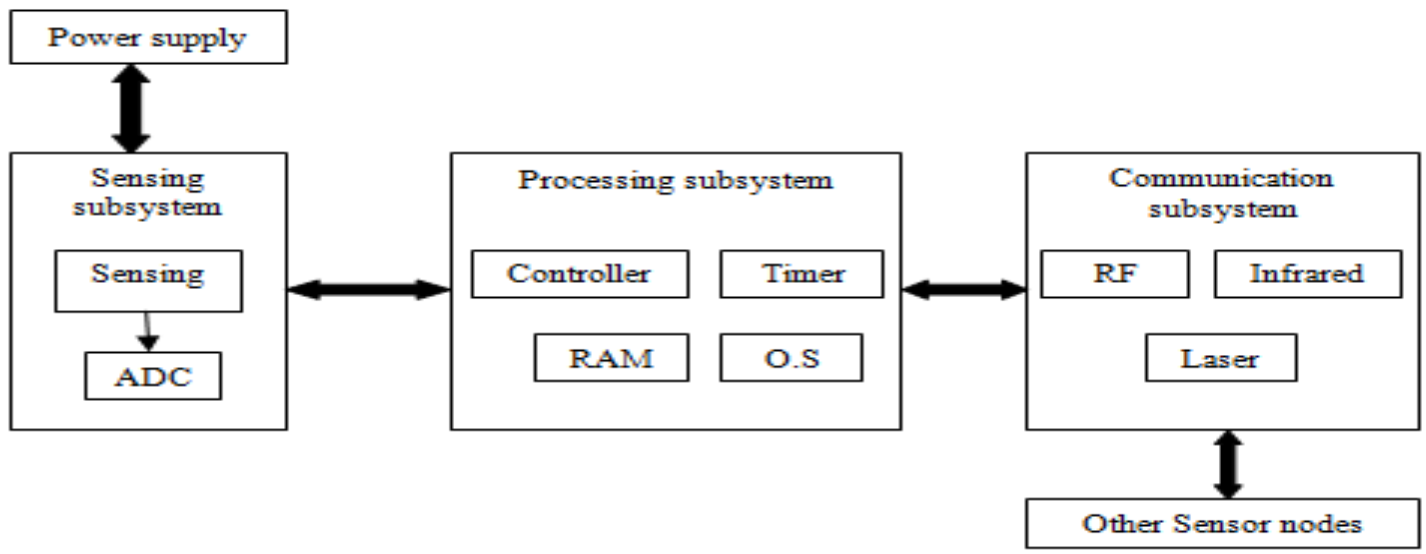
\includegraphics[width=15cm]{2.png}
\caption{c ve d.}
\label{fig:figure3}
\end{figure}
\subsection{e)}
\subsubsection{a...}
Feedback çıkış sinyalinin örneklenmesi ve sonrasında sistemi çalıştıran bir geri dönüş sinyali oluşturmak için girişin geri beslenmesidir. Feedback pozitiftir.
\subsubsection{b...}
R3'ün bağlı olduğu ground'dan dolayı, ve V- ile V+'nin aynı volt değerine sahip olduğu varsayımından ötürü, V+ ucu da V- gibi topraklanmış (0V) kabul edilir. Buna Virtual Ground deriz.Negatif kısma gelen voltaj ile pozitif kısma gelen voltaj birbirine eşit olacağından pozitif kısım da 0V olur. R2’nin olduğu telden ve R1’in olduğu telden KCL yaparsak elimize iki denklem geliyor:
$$\frac{V_{in} - 0}{R_1} = \frac{0-V_{out}}{R_2}$$
olur. $V_{out}$'u çekersek $V_{out}$'un $V_{in}$'e bağlı fonksiyonu
$$V_{out} = -V_{in} \frac{R2}{R1}$$
şeklinde olur.

\section{2 Soru 2}
\subsection{a)}
3 DC voltajını ayrı ayrı değerlendirelim (superposition). V1, V2 ve V3 için Vout'ı ayrı ayrı değerlendirdiğimizde
$$ \frac{V_1 - 0}{RR1} = \frac{-V_o}{R4} $$
$$ \frac{V_2 - 0}{RR2} = \frac{-V_o}{R4} $$
$$ \frac{V_3 - 0}{RR3} = \frac{-V_o}{R4} $$
denklemlerini elde ediyoruz. 3 denklemi de topladığımızda Vo'yu buluyoruz:
$$V_o = - \left(\frac{R4}{RR3} V_3 + \frac{R4}{RR2} V_2 + \frac{R4}{RR1} V_1\right)$$
\subsection{b) }
Devre toplayıcı opamp devresidir. Devre, faz çeviren (inverting) yükselteç gibi çalışmaktadır. a'da bulduğumuz denklemdeki gibi belirli bir oranda (dirençlere göre) V değerlerini topluyor.
\subsection{c) }
\begin{figure}[H]
\centering
\includegraphics[width=15cm]{devre.png}
\caption{Drawed circuit.}
\label{fig:figure3}
\end{figure}
\subsection{d) }
\begin{figure}[H]
\centering
\includegraphics[width=15cm]{v-.png}
\caption{V- ile vout ile kıyaslama sağdaki osiloskop grafiğinde.}
\label{fig:figure3}
\end{figure}

\end{document}